\documentclass[xcolor=tex,dvipsnames]{beamer}  % for hardcopy add 'trans'

\mode<presentation>
{
  \usetheme{Singapore}
  % or ...
  \setbeamercovered{transparent}
  % or whatever (possibly just delete it)
}


\usepackage{fontspec} 
\usepackage[mathscr]{euscript} 
%\usepackage[xcharter]{newtxmath}
%\setmainfont{XCharter}
\setmonofont{DejaVu Sans Mono}[Scale=MatchLowercase] % provides unicode characters 


\usefonttheme{professionalfonts}
%\usepackage[english]{babel}
% or whatever
%\usepackage[latin1]{inputenc}
% or whatever
%\usepackage{times}
\usepackage[T1]{fontenc}
% Or whatever. Note that the encoding and the font should match. If T1
% does not look nice, try deleting the line with the fontenc.

%%%%%%%%%%%%%%%%%%%%%% start my preamble %%%%%%%%%%%%%%%%%%%%%%
\renewcommand{\insertnavigation}[1]{}

\addtobeamertemplate{navigation symbols}{}{%
    \usebeamerfont{footline}%
    \usebeamercolor[fg]{footline}%
    \hspace{1em}%
    \insertframenumber/\inserttotalframenumber
}

\setbeamercolor{footline}{fg=blue}
\setbeamerfont{footline}{series=\bfseries}

%\setbeamertemplate{mini frames}{}

\usepackage{adjustbox}

\usepackage{graphicx}
\usepackage{amsmath, amssymb, amsthm}

\usepackage{fancyvrb}

\usepackage{hyperref}

% fonts, caligraphic
\usepackage{mathpazo}
%\usepackage{mathrsfs}
\usepackage{bbm}

% tikz
\usepackage{tikz}
\usetikzlibrary{positioning}
\usetikzlibrary{arrows}
\usetikzlibrary{calc}
\usetikzlibrary{intersections}
\usetikzlibrary{matrix}
\usetikzlibrary{decorations}
\usepackage{pgf}
\usepackage{pgfplots}
\usetikzlibrary{shapes, fit}

% from fazeleh
\usetikzlibrary{arrows.meta}

%\usetikzlibrary{arrows.meta}
\usetikzlibrary{decorations.pathreplacing}  %for brac



\usepackage{graphviz}

%\usepackage[usenames, dvipsnames]{color}


% nice inequalities
\renewcommand{\leq}{\leqslant}
\renewcommand{\geq}{\geqslant}


\setlength{\parskip}{1.5ex plus0.5ex minus0.5ex}
\setlength{\jot}{12pt} 

\usepackage[ruled, lined]{algorithm2e}


\definecolor{pale}{RGB}{235, 235, 235}
\definecolor{pale2}{RGB}{175,238,238}
\definecolor{turquois4}{RGB}{0,134,139}
\definecolor{DarkOrange1}{RGB}{255,127,0}

\newcommand{\emp}[1]{\textcolor{DarkOrange1}{\bf #1}}
\newcommand{\newtopic}[1]{\textcolor{Green}{\Large \bf #1}}
\newcommand{\navy}[1]{\textcolor{Blue}{\bf #1}}
\newcommand{\navymth}[1]{\textcolor{Blue}{#1}}
\newcommand{\red}[1]{\textcolor{red}{#1}}
\newcommand{\brown}[1]{\textcolor{Brown}{\sf #1}}
\newcommand{\green}[1]{\textcolor{ForestGreen}{\sf #1}}

% Minted
\definecolor{bg}{rgb}{0.95,0.95,0.95}
\usepackage{minted}
\usemintedstyle{friendly}
\newminted{python}{mathescape,frame=lines,framesep=4mm,bgcolor=bg}
\newminted{ipython}{mathescape,frame=lines,framesep=4mm,bgcolor=bg}
\newminted{julia}{mathescape,frame=lines,framesep=4mm,bgcolor=bg}
\newminted{c}{mathescape,frame=lines,framesep=4mm,bgcolor=bg}
\renewcommand{\theFancyVerbLine}{\sffamily
    \textcolor[rgb]{0.5,0.5,1.0}{\scriptsize {\arabic{FancyVerbLine}}}}


\newcommand{\Fact}{\textcolor{Brown}{\bf Fact. }}
\newcommand{\Facts}{\textcolor{Brown}{\bf Facts }}
\newcommand{\keya}{\textcolor{turquois4}{\bf Key Idea. }}
\newcommand{\Factnodot}{\textcolor{Brown}{\bf Fact }}
\newcommand{\Eg}{\textcolor{ForestGreen}{Example. }}
\newcommand{\Egs}{\textcolor{ForestGreen}{Examples. }}
\newcommand{\Ex}{{\bf Ex. }}



\newcommand{\CC}{\mathbbm C}
\newcommand{\EE}{\mathbbm E}
\newcommand{\FF}{\mathbbm F}
\newcommand{\RR}{\mathbbm R}
\newcommand{\KK}{\mathbbm K}
\newcommand{\MM}{\mathbbm M}
\newcommand{\NN}{\mathbbm N}
\newcommand{\PP}{\mathbbm P}
\newcommand{\TT}{\mathbbm T}
\newcommand{\QQ}{\mathbbm Q}
\newcommand{\WW}{\mathbbm W}
\newcommand{\VV}{\mathbbm V}
\newcommand{\ZZ}{\mathbbm Z}

\newcommand{\Asf}{\mathsf A}
\newcommand{\Esf}{\mathsf E}
\newcommand{\Fsf}{\mathsf F}
\newcommand{\Gsf}{\mathsf G}
\newcommand{\Msf}{\mathsf M}
\newcommand{\Lsf}{\mathsf L}
\newcommand{\Nsf}{\mathsf N}
\newcommand{\Psf}{\mathsf P}
\newcommand{\Qsf}{\mathsf Q}
\newcommand{\Ssf}{\mathsf S}
\newcommand{\Tsf}{\mathsf T}
\newcommand{\Xsf}{\mathsf X}
\newcommand{\Ysf}{\mathsf Y}
\newcommand{\Vsf}{\mathsf V}
\newcommand{\Wsf}{\mathsf W}
\newcommand{\Zsf}{\mathsf Z}

\newcommand{\aA}{\mathscr A}
\newcommand{\bB}{\mathscr B}
\newcommand{\cC}{\mathscr C}
\newcommand{\dD}{\mathscr D}
\newcommand{\eE}{\mathscr E}
\newcommand{\gG}{\mathscr G}
\newcommand{\hH}{\mathscr H}
\newcommand{\iI}{\mathscr I}
\newcommand{\fF}{\mathscr F}
\newcommand{\lL}{\mathscr L}
\newcommand{\pP}{\mathscr P}
\newcommand{\rR}{\mathscr R}
\newcommand{\sS}{\mathscr S}
\newcommand{\vV}{\mathscr V}
\newcommand{\wW}{\mathscr W}
\newcommand{\mM}{\mathscr M}
\newcommand{\oO}{\mathscr O}
\newcommand{\zZ}{\mathscr Z}

\newcommand{\bP}{\mathbf P} 
\newcommand{\bR}{\mathbf R}
\newcommand{\bQ}{\mathbf Q}


%%%%%% special symbols %%%%%%%%%%

\newcommand{\volone}{Volume~I}
\newcommand{\voltwo}{Volume~II}

% transpose, not currently using
\newcommand\T{{\mathpalette\raiseT\intercal}}
\newcommand\raiseT[2]{\raisebox{0.25ex}{$#1#2$}}

% nice inequalities
\renewcommand{\leq}{\leqslant}
\renewcommand{\geq}{\geqslant}

% nice greek letters
\renewcommand{\phi}{\varphi}
\renewcommand{\epsilon}{\varepsilon}

% inner product
\providecommand{\inner}[1]{\left\langle{#1}\right\rangle}

% set of matrices
\newcommand{\matset}[2]{ \MM^{ #1 \times #2 } }

% stochastic dominance
\newcommand{\lefsd}{\preceq_{\textrm{F}}}
\newcommand{\lessd}{\preceq_{\textrm{S}}}

% argmax and min
\newcommand{\argmax}{\operatornamewithlimits{argmax}}
\newcommand{\argmin}{\operatornamewithlimits{argmin}}

% sets and logic
\newcommand{\st}{\ensuremath{\ \mathrm{s.t.}\ }}
\newcommand{\setntn}[2]{ \{ #1 : #2 \} }
\newcommand{\natset}[1]{[ #1 ]}

% some useful symbols
\newcommand{\given}{\, | \,}
\newcommand{\cf}[1]{ \lstinline|#1| }
\newcommand{\fore}{\therefore \quad}
\newcommand{\1}{\mathbbm 1}
\newcommand{\me}{\mathrm{e}}               % Euler's e
\newcommand*\diff{\mathop{}\!\mathrm{d}}   % d for integrals

% shortcuts
\newcommand{\la}{\langle}
\newcommand{\ra}{\rangle}

% relations
\newcommand{\eqdist}{\stackrel{d} {=} }
\newcommand{\iidsim}{\stackrel{\textrm{ {\sc iid }}} {\sim} }

% convergence
\newcommand{\tod}{\stackrel { d } {\to} }
\newcommand{\tow}{\stackrel { w } {\to} }
\newcommand{\toprob}{\stackrel { p } {\to} }
\newcommand{\toms}{\stackrel { ms } {\to} }


%%%%%%%%%%% operators %%%%%%%%%%%%

\DeclareMathOperator{\Exp}{Exp}  % exponential draw
\DeclareMathOperator{\Lip}{Lip}
\DeclareMathOperator{\cl}{cl}
\DeclareMathOperator{\graph}{graph}
\DeclareMathOperator{\interior}{int}
\DeclareMathOperator{\Prob}{Prob}
\DeclareMathOperator{\determinant}{det}
\DeclareMathOperator{\trace}{trace}
\DeclareMathOperator{\sgn}{sgn}
\DeclareMathOperator{\Span}{span}
\DeclareMathOperator{\diag}{diag}
\DeclareMathOperator{\proj}{proj}
\DeclareMathOperator{\rank}{rank}
\DeclareMathOperator{\kernel}{null}
\DeclareMathOperator{\cov}{Cov}
\DeclareMathOperator{\corr}{Corr}
\DeclareMathOperator{\var}{Var}
\DeclareMathOperator{\mse}{mse}
\DeclareMathOperator{\se}{se}
\DeclareMathOperator{\range}{range}
\DeclareMathOperator{\dimension}{dim}
\DeclareMathOperator{\epi}{epi}
\DeclareMathOperator{\vecop}{vec}

\DeclareMathOperator{\real}{Re}
\DeclareMathOperator{\imag}{Im}

\DeclareMathOperator{\csum}{cs} % column sum
\DeclareMathOperator{\rsum}{rs} % row sum



\hypersetup{
    linkcolor=Blue,
    colorlinks=true,
    filecolor=magenta,      % color of file links
    urlcolor=cyan           % color of external links
}


%\pgfdeclareimage[height=1.2cm]{university-logo}{../tuxswatter2}
%\logo{\pgfuseimage{university-logo}}

%\addtobeamertemplate{headline}{}
%{%
%\begin{flushright}
%\begin{tikzpicture}[remember picture,overlay]
%\node [left ]{\includegraphics[width=0.5cm]{../tuxswatter2.png}};
%\end{tikzpicture}
%\end{flushright}
%\vskip -0.1cm
%} 

 \date[\today]{}

\title{CBC QuantEcon Workshop}







\subtitle{Introduction}

\author{John Stachurski}


\date{September 2022}


\begin{document}

\begin{frame}
  \titlepage
\end{frame}





\section{Introduction}


\begin{frame}
    \frametitle{Instructors}

    \navy{John Stachurski}

    \begin{itemize}
        \item Researcher in asset pricing, dynamic programming, Markov process theory
        \item Co-founder of QuantEcon
        \item Based at Australian National University
    \end{itemize}

        \vspace{0.5em}
        \vspace{0.5em}

    \navy{Pablo Winant}

    \begin{itemize}
        \item Researcher in macroeconomics and computational methods
        \item CREST and ESCP Business School
        \item Lead developer of \texttt{dolo}, \texttt{interpolation}, \texttt{NoLib}
    \end{itemize}

\end{frame}

\begin{frame}

    \navy{Schedule}

    \begin{itemize}
        \item September 20th - 23rd: Scientific computing with Python
        \item September 24th - 25th: Weekend break
        \item September 26th - 27th: Scientific computing with Julia
    \end{itemize}

        \vspace{0.5em}
        \vspace{0.5em}
    \navy{Format}

    \begin{itemize}
        \item 08:30 - 10:30: Lecture
        \item 10:30 - 11:00: Coffee Break
        \item 11:00 - 13:00: Practice Sessions
        \item 14:30 - 16:00: Office hours
    \end{itemize}

\end{frame}


\begin{frame}
    \frametitle{Content: Python Workshop}


    \begin{itemize}
        \item Introduction to scientific computing with Python
        \vspace{0.5em}
        \vspace{0.5em}
        \item Dynamics (simulation, Markov chains)
        \vspace{0.5em}
        \vspace{0.5em}
        \item Fixed points and job search 
        \vspace{0.5em}
        \vspace{0.5em}
        \item Dynamic programming: theory and algorithms
        \vspace{0.5em}
        \vspace{0.5em}
        \item Parallelization on the GPU 
    \end{itemize}

\end{frame}




\begin{frame}


    Assumptions:

    \begin{itemize}
        \item Some familiarity with programming / computation
        \vspace{0.3em}
        \vspace{0.3em}
        \item linear algebra, multivariate calculus, etc.
        \vspace{0.3em}
        \vspace{0.3em}
        \item have seen some dynamic programming
    \end{itemize}

        \vspace{0.3em}
        \vspace{0.3em}
        \vspace{0.3em}
        \vspace{0.3em}
        \vspace{0.3em}
    Resources:

    \begin{itemize}
        \item \url{https://github.com/QuantEcon/cbc_workshops}
    \end{itemize}


\end{frame}




\section{Overview}


\begin{frame}
    \frametitle{Background}

    The theme of Part 1 is economic modeling Python


        \vspace{0.3em}
        \vspace{0.3em}
        \vspace{0.3em}
        \vspace{0.3em}
    Why use Python for economic modeling?

        \vspace{0.3em}
        \vspace{0.3em}
        \vspace{0.3em}
        \vspace{0.3em}
    In fact, why use Python for scientific computing?

        \vspace{0.3em}
        \vspace{0.3em}
        \vspace{0.3em}
        \vspace{0.3em}
    Let's compare Python to some of the alternatives

\end{frame}





\begin{frame}
    \frametitle{Language Types}
    
    \navy{Low level } 
    
    \begin{itemize}
        \item C/C++
        \item Fortran
        \item assembly
    \end{itemize}

    \vspace{1em}

    \navy{High level } 

    \begin{itemize}
        \item Python
        \item Ruby
        \item TypeScript
    \end{itemize}

\end{frame}




\begin{frame}[fragile]

    Low level languages give us fine grained control 
    
    \Eg \brown{1 + 1} in assembly

    {\small
    \begin{minted}{as}
pushq   %rbp
movq    %rsp, %rbp
movl    $1, -12(%rbp)
movl    $1, -8(%rbp)
movl    -12(%rbp), %edx
movl    -8(%rbp), %eax
addl    %edx, %eax
movl    %eax, -4(%rbp)
movl    -4(%rbp), %eax
popq    %rbp
    \end{minted}
    }



\end{frame}


\begin{frame}
    
    \navy{High level languages} give us abstraction, automation, etc.

\end{frame}



\begin{frame}[fragile]

    \Eg Reading from a file in Python
    
    \begin{minted}{python}
    data_file = open("data.txt")
    for line in data_file:
        print(line.capitalize()) 
    data_file.close()
    \end{minted}

\end{frame}


\begin{frame}
    \frametitle{Trade-Offs}

    \begin{figure}
       \begin{center}
        \scalebox{.36}{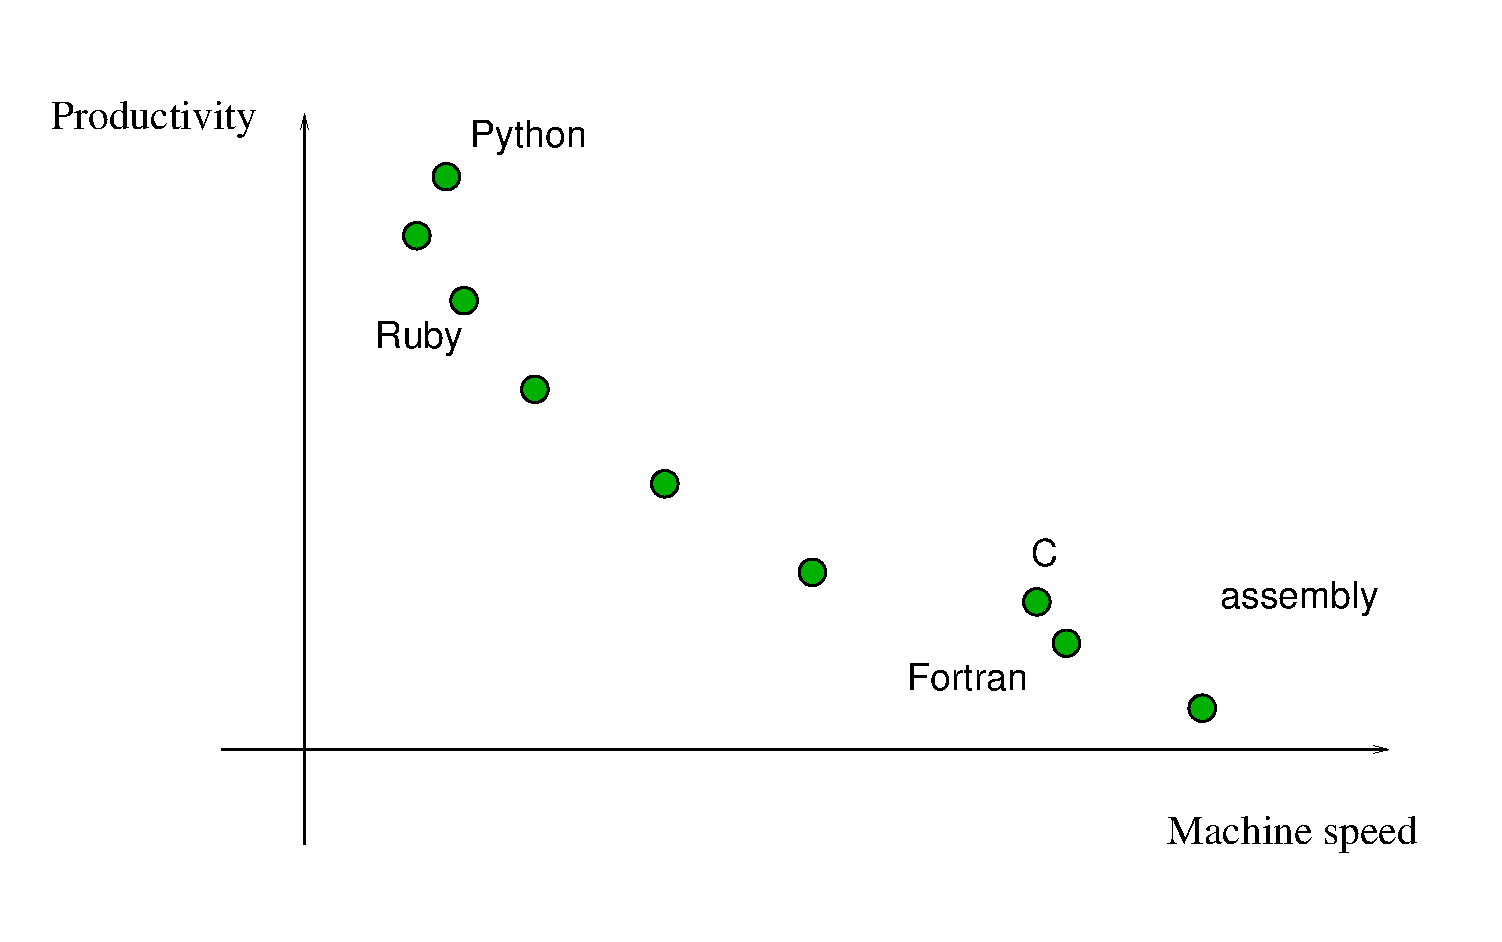
\includegraphics{tradeoff.pdf}}
       \end{center}
    \end{figure}

\end{frame}



\begin{frame}[fragile]
    \frametitle{But what about scientific computing?}
    
    \navy{Requirements}

    \begin{itemize}
        \item \underline{\green{Productive}} --- easy to read, write, debug, explore
            \vspace{0.4em}
            \vspace{0.4em}
            \vspace{0.4em}
        \item \underline{\green{Fast}} computations
    \end{itemize}

\end{frame}




\begin{frame}
    \frametitle{Trade-Offs}

    \begin{figure}
       \begin{center}
        \scalebox{.36}{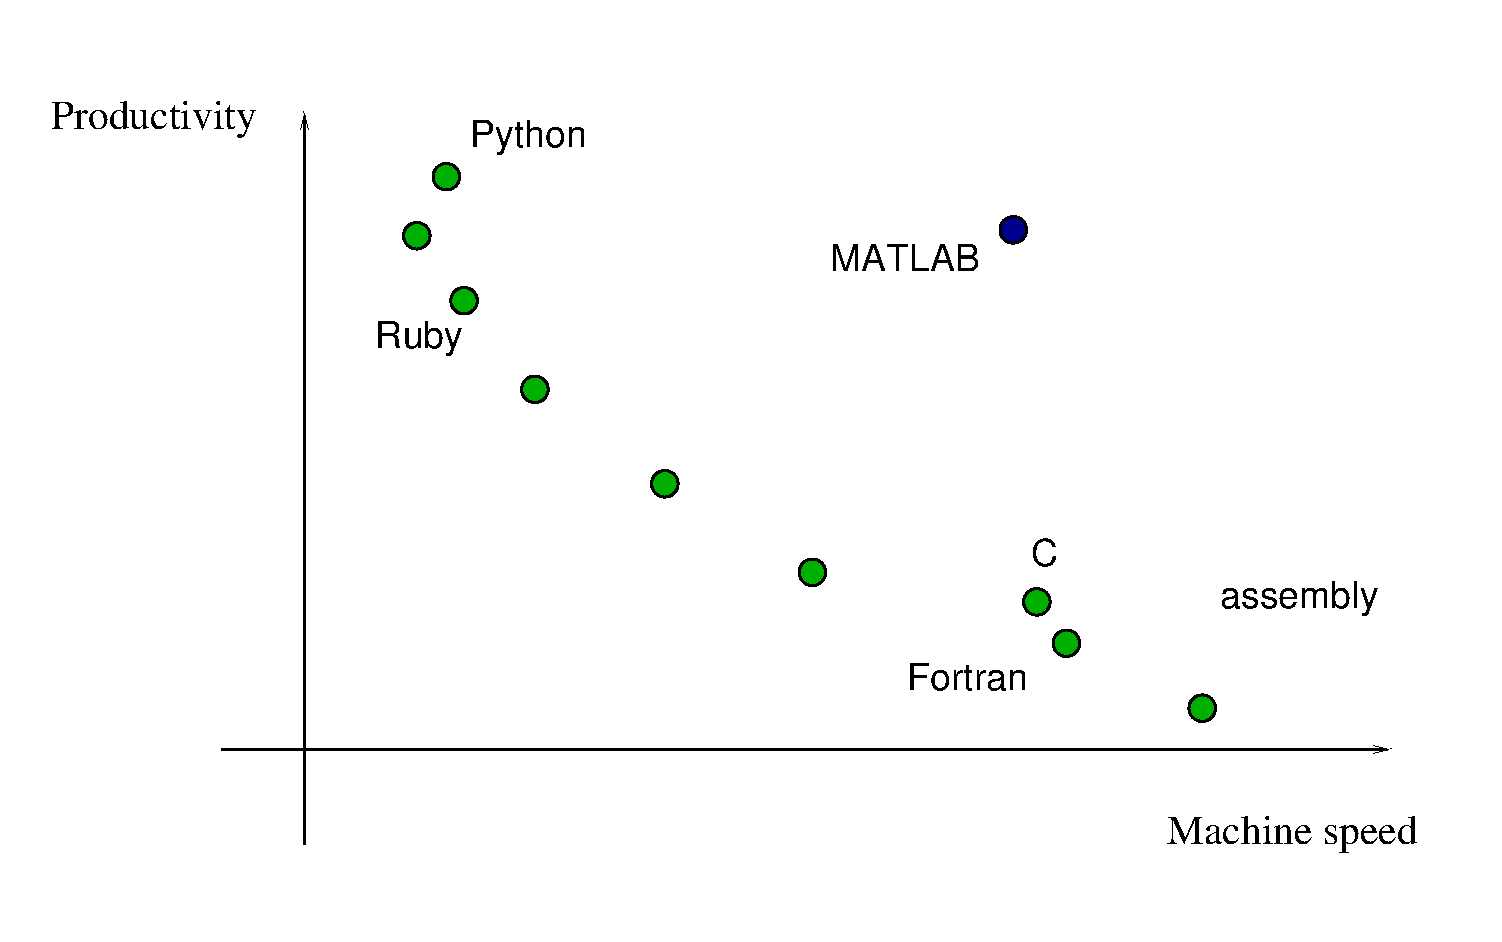
\includegraphics{tradeoff2.pdf}}
       \end{center}
    \end{figure}

\end{frame}


\begin{frame}
    \frametitle{Trade-Offs}

    \begin{figure}
       \begin{center}
        \scalebox{.36}{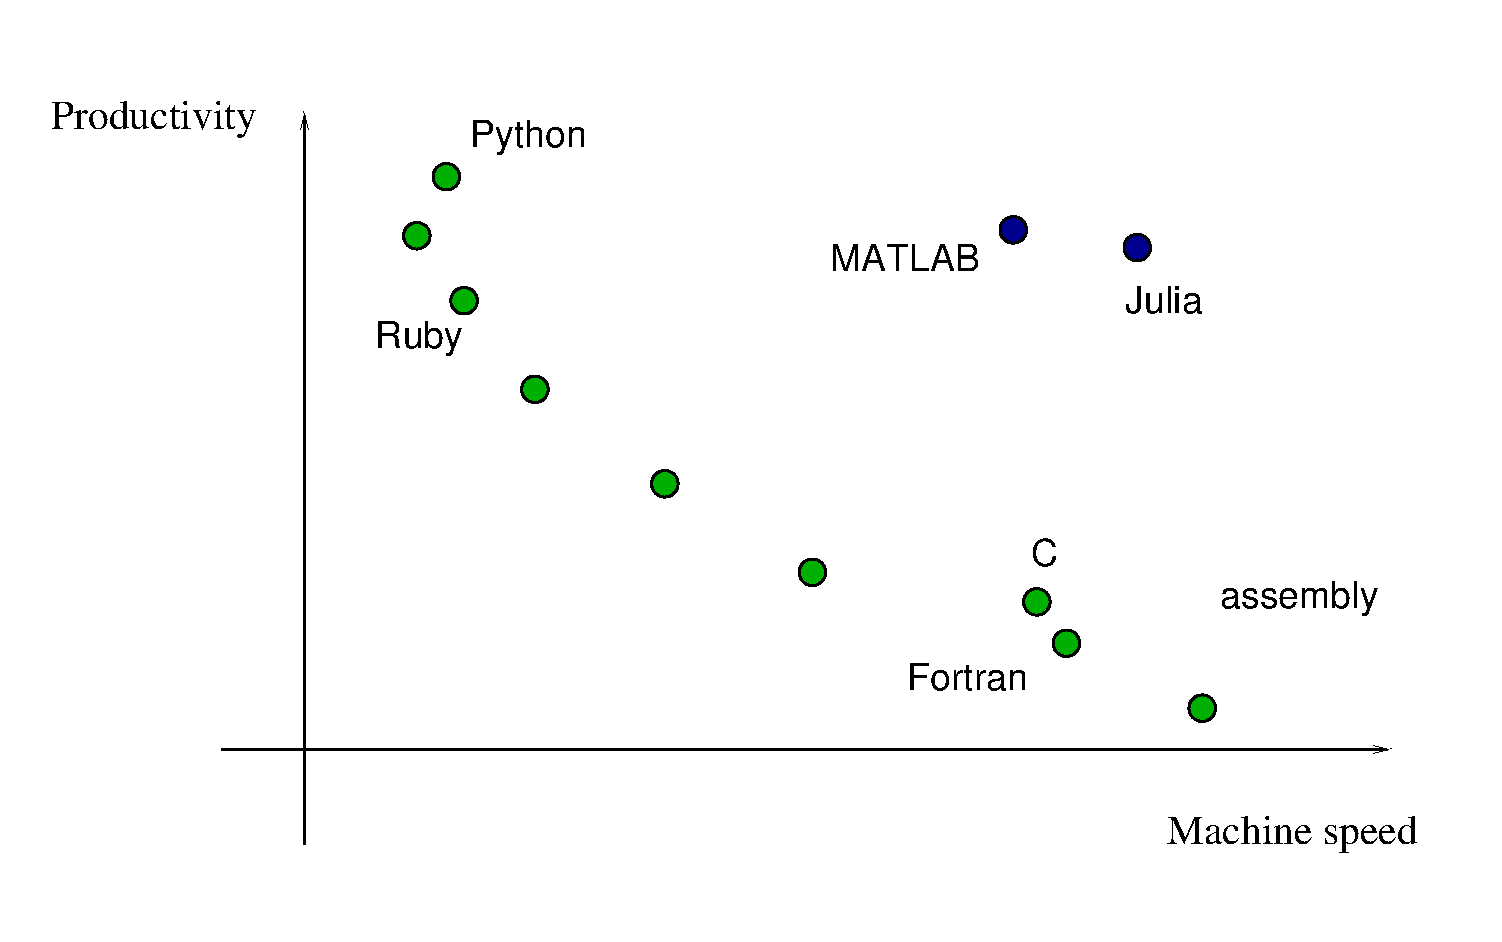
\includegraphics{tradeoff3.pdf}}
       \end{center}
    \end{figure}

\end{frame}


\begin{frame}
    \frametitle{Trade-Offs}

    \begin{figure}
       \begin{center}
        \scalebox{.36}{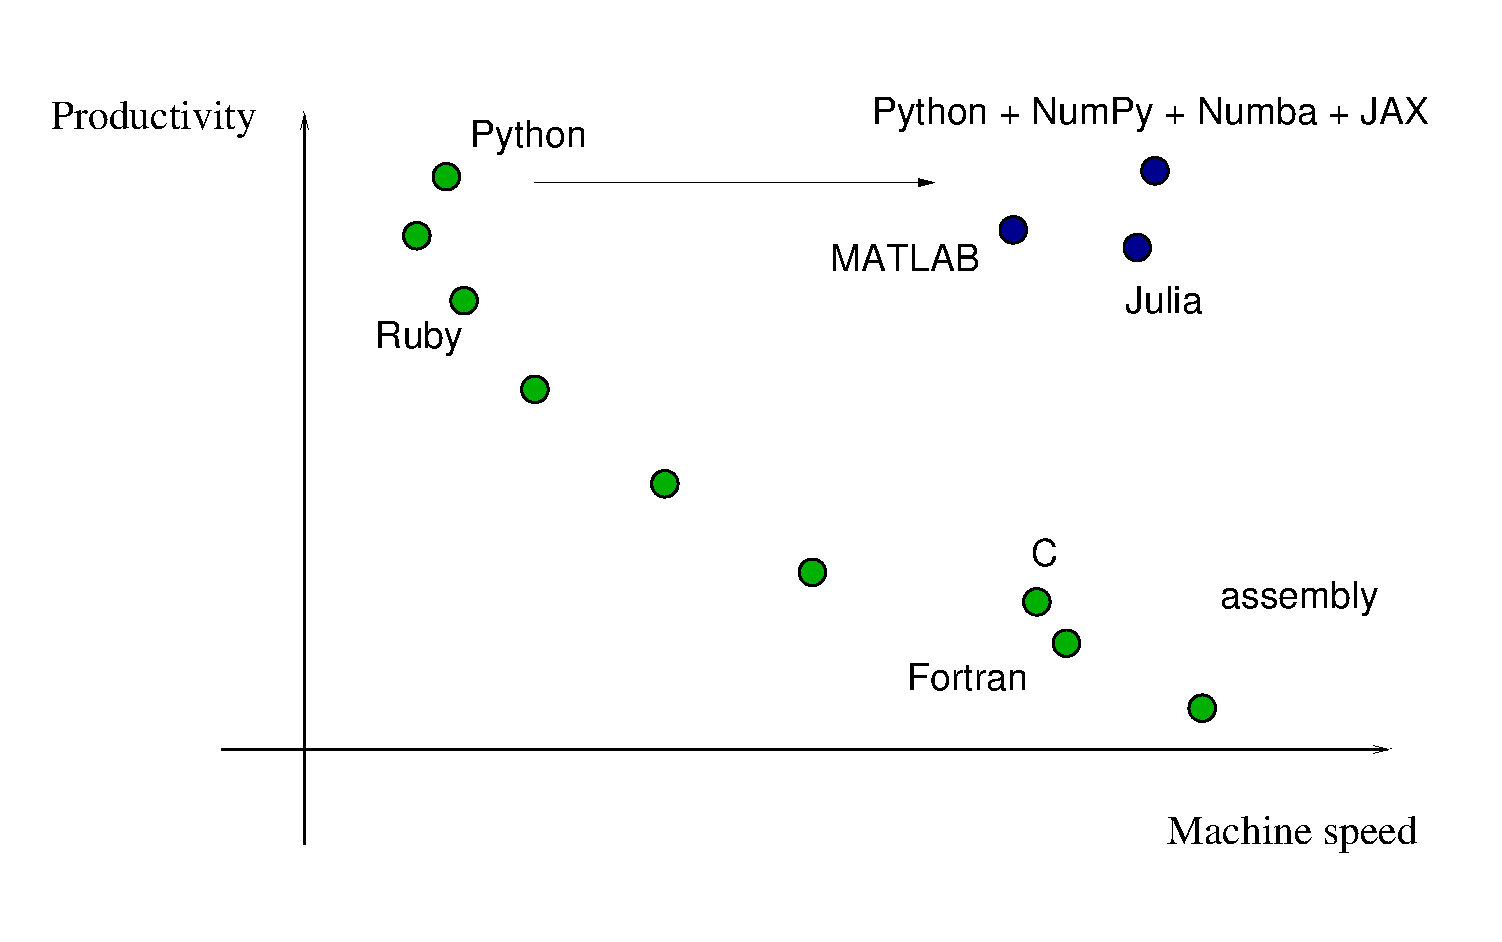
\includegraphics{tradeoff4.pdf}}
       \end{center}
    \end{figure}

\end{frame}




\section{Which Language?}


\begin{frame}
    \frametitle{Which Language}


    How about R?
    \vspace{0.5em}

    \begin{itemize}
        \item Specialized to statistics
            \vspace{0.5em}
        \item Easy to learn, well designed
            \vspace{0.5em}
        \item Huge range of estimation routines
            \vspace{0.5em}
        \item Significant demand for R programmers
            \vspace{0.5em}
        \item Popular in academia 
    \end{itemize}

\end{frame}


\begin{frame}
    
    Loosing some ground to Python
            \vspace{0.5em}
            \vspace{0.5em}
            \vspace{0.5em}

    \Eg Chris Wiggins, Chief Data Scientist at The New York Times:

            \vspace{0.5em}
     ``Python has gotten sufficiently weapons grade that we don't descend into
     R anymore. Sorry, R people. I used to be one of you but we no longer
     descend into R.''


\end{frame}


\begin{frame}
    \frametitle{Julia}

    Pros:
    
    \begin{itemize}
        \item Fast and elegant
            \vspace{0.5em}
        \item Many scientific routines
            \vspace{0.5em}
        \item Julia is written in Julia
    \end{itemize}

            \vspace{0.5em}
            \vspace{0.5em}
            \vspace{0.5em}
    Cons:
    
    \begin{itemize}
        \item More niche than Python
            \vspace{0.5em}
        \item Yet to achieve rapid growth
    \end{itemize}

\end{frame}




\begin{frame}
    \frametitle{Python}

    Pros:
    
    \begin{itemize}
        \item Massive scientific ecosystem
            \vspace{0.5em}
        \item Strong investment from Google, Facebook (Meta), etc.
            \vspace{0.5em}
        \item Huge demand for tech-savvy Python programmers
    \end{itemize}


            \vspace{0.5em}
            \vspace{0.5em}
    Cons:
    
    \begin{itemize}
        \item Numerical code not as clean as Julia
            \vspace{0.5em}
        \item Econometrics libraries less developed than R/STATA
    \end{itemize}

\end{frame}




%\begin{frame}
    %\frametitle{Scientific Computing}
    
    %Python has strong tools in vectorization / JIT compilation /
    %parallelization / visualization / etc.

    %Examples:

    %\begin{itemize}
        %\item SciPy, NumPy, Matplotlib, pandas
            %\vspace{0.5em}
        %\item Numba (JIT compilation, multithreading)
            %\vspace{0.5em}
        %\item Tensorflow, PyTorch (machine learning, AI)
            %\vspace{0.5em}
        %\item JAX (JIT compilation, parallelization), etc., etc.
    %\end{itemize}

%\end{frame}

\begin{frame}
    

    Popularity, others vs \underline{one} Python library (pandas)

    \begin{figure}
       \begin{center}
        \scalebox{.4}{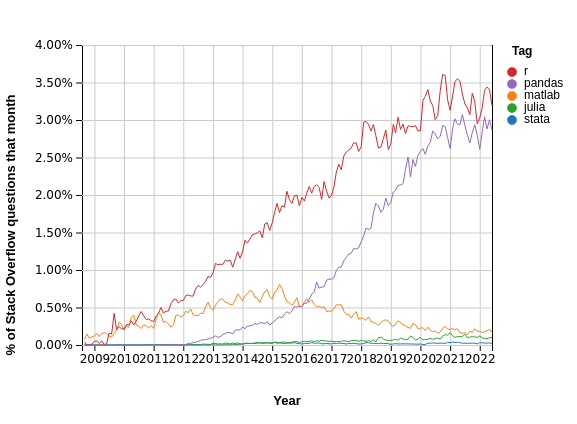
\includegraphics{python_vs_rest.png}}
       \end{center}
    \end{figure}


\end{frame}






\section{Trends}

\begin{frame}
    \frametitle{Current Trend 1: Parallelization}

    CPU frequency (clock speed) growth is slowing

    \begin{figure}
       \begin{center}
        \scalebox{.22}{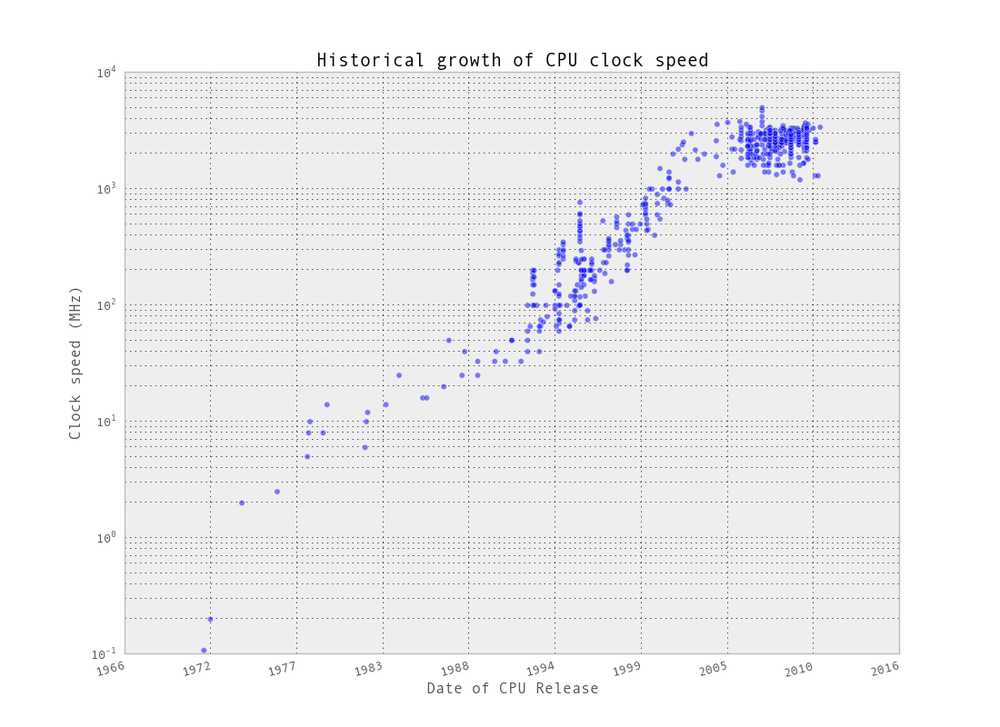
\includegraphics{processor_clock.png}}
       \end{center}
    \end{figure}

\end{frame}


\begin{frame}
    
    Chip makers have responded by developing multi-core processors

    \begin{figure}
       \begin{center}
        \scalebox{.2}{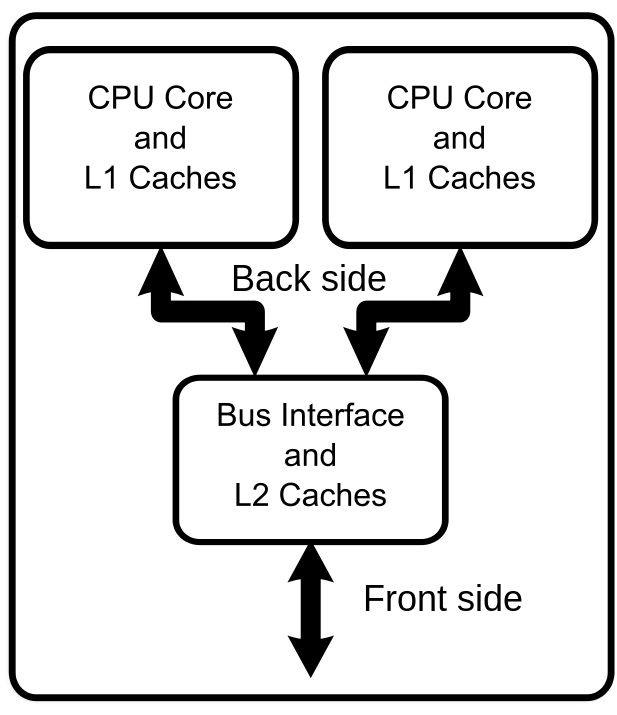
\includegraphics{dual_core.png}}
       \end{center}
    \end{figure}

    Source: Wikipedia


\end{frame}


\begin{frame}

    \navy{GPUs / TPUs} are becoming more and more important


    \begin{figure}
       \begin{center}
        \scalebox{.14}{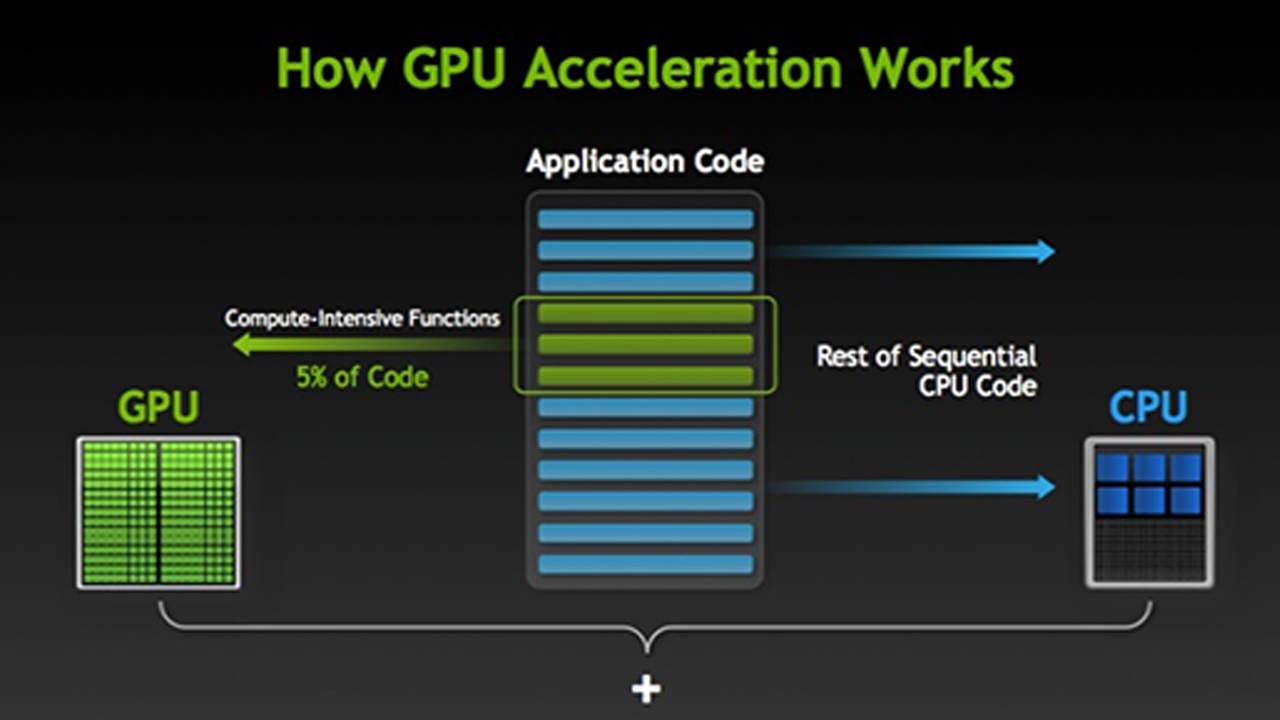
\includegraphics{gpu.jpg}}
       \end{center}
    \end{figure}

    \vspace{0.5em}

    Applications: 
    \begin{itemize}
        \item machine learning, deep learning, etc.
        \item dynamic programming!
    \end{itemize}
    

\end{frame}



\begin{frame}
    \frametitle{Trend 2: Distributed Computing}
    
    Advantages: 
    %
    \begin{itemize}
        \item run code on big machines we don't have to buy
        \vspace{0.5em}
        \item circumvent internal IT departments
    \end{itemize}

    \vspace{0.5em}

    Options:
    %
    \begin{itemize}
        \item Google Colab, PythonAnywhere, etc.
            \vspace{0.5em}
        \item AWS 
            \vspace{0.5em}
        \item Supercomputers
    \end{itemize}

\end{frame}






\section{Set Up}







\begin{frame}
    \frametitle{Downloads / Installation / Remote Options}

    \green{Install Python + scientific libraries (optional)}
    
    \begin{itemize}
        \item Install Anaconda from {\footnotesize \url{https://www.anaconda.com/}}
        \vspace{0.5em}
            \begin{itemize}
                \item Select latest version 
                \item For your OS
                \item Say ``yes'' at prompts
            \end{itemize}
        \vspace{0.5em}
        \item Not plain vanilla Python
    \end{itemize}


    \vspace{1em}

    \green{Remote options}

    \begin{itemize}
        \item \url{https://colab.research.google.com}
    \end{itemize}


\end{frame}



\begin{frame}
    \frametitle{Notebooks}

    Now let's move on to
    %
    \begin{itemize}
        \item \texttt{python\_by\_example.ipynb}
        \item \texttt{finite\_markov.ipynb}
        \item \texttt{equilibrium.ipynb}
        \item \texttt{numba.ipynb}
        \item \texttt{european\_option\_numba.ipynb}
    \end{itemize}

\end{frame}





\end{document}


